\PassOptionsToPackage{xetex}{xcolor}
\PassOptionsToPackage{xetex}{graphicx}
\documentclass[a4paper,landscape,headrule,footrule,xetex]{foils}

%%
%%%  Macros
%%%
\newcommand{\logo}{~}
\MyLogo{HG2052 (2020)}
%\newcommand{\Story}{\SHA{HOUN}{The Hound of the Baskervilles}}

\newcommand{\header}[3]{%
\title{\vspace*{-2ex} \Large HG2052
\\\large  Language, Technology and the Internet
\\[2ex] \Large  \emp{#2}}
\author{\blu{Francis Bond}   \\ 
\normalsize  \textbf{Division of Linguistics and Multilingual Studies}\\
\normalsize  \url{http://www3.ntu.edu.sg/home/fcbond/}\\
\normalsize  \texttt{bond@ieee.org}}
\MyLogo{HG2052 (2020)}
\date{#1}
\renewcommand{\logo}{#2}
 \hypersetup{
   pdfinfo={
     Author={Francis Bond},
     Title={#1: #2},
     Subject={HG2052: Language, Technology and the Internet},
     Keywords={Language, Technology, Internet},
     License={CC BY 4.0}
   }
 %  pdfcopyright={Copyright © Francis Bond. Creative Commons 4.0 Attribution License.}
 %  pdflicenseurl={http://creativecommons.org/licenses/by/4.0/}
 }
}


%%
%% Multilingual Stuff
%%
\usepackage[a4paper,landscape,margin=25mm]{geometry}

\usepackage{fontenc}
\usepackage{polyglossia}
\setmainlanguage{english}
\setmainfont{TeX Gyre Pagella}
%\setmainfont{Linux Libertine}
%\setmainfont{Charis SIL}
\newfontfamily{\ipafont}{Gentium}
\newcommand{\ipa}[1]{{\ipafont\selectfont #1}}
\usepackage{xeCJK}

\setCJKmainfont{Noto Sans CJK SC}
\setCJKsansfont{Noto Sans CJK SC}
%\setCJKttfont{Noto Sans CJK SC}
%\setCJKmainfont{WenQuanYi Micro Hei}
%\clearpage
%\setCJKmainfont{AR PL SungtiL GB}

\usepackage[xetex]{xcolor}
\usepackage[xetex]{graphicx}
\newcommand{\blu}[1]{\textcolor{blue}{#1}}
\newcommand{\grn}[1]{\textcolor{green}{#1}}
\newcommand{\hide}[1]{\textcolor{white}{#1}}
\newcommand{\emp}[1]{\textcolor{red}{#1}}
\newcommand{\txx}[1]{\textbf{\textcolor{blue}{#1}}}
\newcommand{\lex}[1]{\textbf{\mtcitestyle{#1}}}

\usepackage{pifont}
\renewcommand{\labelitemi}{\textcolor{violet}{\ding{227}}}
\renewcommand{\labelitemii}{\textcolor{purple}{\ding{226}}}

\newcommand{\subhead}[1]{\noindent\textbf{#1}\\[5mm]}

\newcommand{\Bad}{\emp{\raisebox{0.15ex}{\ensuremath{\mathbf{\otimes}}}}}
\newcommand{\bad}{*}

\newcommand{\com}[1]{\hfill \textnormal{(\emp{#1})}}%
\newcommand{\cxm}[1]{\hfill \textnormal{(\txx{#1})}}%
\newcommand{\cmm}[1]{\hfill \textnormal{(#1)}}%
\usepackage{amssymb}
\usepackage{relsize,xspace}
\newcommand{\into}{\ensuremath{\rightarrow}\xspace}
\newcommand{\ent}{\ensuremath{\Rightarrow}\xspace}
\newcommand{\nent}{\ensuremath{\not\Rightarrow}\xspace}
\newcommand{\tot}{\ensuremath{\leftrightarrow}\xspace}
\usepackage{url}
\usepackage[hidelinks]{hyperref}
\hypersetup{
     colorlinks,
     linkcolor={blue!50!black},
     citecolor={red!50!black},
     urlcolor={blue!80!black}
}
%\usepackage{hyperxmp}
\usepackage{url}
\newcommand{\lurl}[1]{\MyLogo{\url{#1}}}

\usepackage{mygb4e}
\let\eachwordone=\itshape
\newcommand{\lx}[1]{\textbf{\textit{#1}}}
\newcommand{\ix}{\ex\it}

\newcommand{\cen}[2]{\multicolumn{#1}{c}{#2}}
%\usepackage{times}
%\usepackage{nttfoilhead}
\newcommand{\myslide}[1]{%
\foilhead[-25mm]{\raisebox{12mm}[0mm]{\emp{#1}}}%
\leftheader{}%
\MyLogo{\logo}}

\newcommand{\mytask}[1]{%
\foilhead[-25mm]{\raisebox{12mm}[0mm]{\emp{#1}}}
\leftheader{🔍 Hi}%
\MyLogo{\logo}}

\newcommand{\myslider}[1]{\rotatefoilhead[-25mm]{\raisebox{12mm}[0mm]{\emp{#1}}}}
%\newcommand{\myslider}[1]{\rotatefoilhead{\raisebox{-8mm}{\emp{#1}}}}

\newcommand{\section}[1]{\myslide{}{\begin{center}\Huge \emp{#1}\end{center}}}

\usepackage{tcolorbox}
% \newcommand{\task}{\marginpar{\raisebox{-1ex}{\large
%       \tcbox[colframe=red,colback=white,arc=3pt]{\textbf{?}}}}}
% \newcommand{\task}{\marginpar{\raisebox{-1ex}{
%       \hspace{-0.5em}\tcbox[colframe=red,colback=white,arc=3pt]{%
%         \includegraphics[width=1.5em]{pics/detective}}}}}
\newcommand{\task}{\marginpar{\raisebox{-2ex}{
      \hspace{-0.5em}\reflectbox{\includegraphics[width=2em]{pics/detective}}}}}

\usepackage[lyons,j,e,k]{mtg2e}
\renewcommand{\mtcitestyle}[1]{\textcolor{teal}{\textsl{#1}}}
%\renewcommand{\mtcitestyle}[1]{\textsl{#1}}
\newcommand{\chn}{\mtciteform}
\newcommand{\cmn}{\mtciteform}
\newcommand{\iz}[1]{\textup{\texttt{\textcolor{blue}{\textbf{#1}}}}}
\newcommand{\con}[1]{\textsc{#1}}
\newcommand{\gm}{\textsc}
\newcommand{\cmp}[1]{{[\textsc{#1}]}}
\newcommand{\sr}[1]{\ensuremath{\langle}#1\ensuremath{\rangle}}
\usepackage[normalem]{ulem}
\newcommand{\ul}{\uline}
\newcommand{\uul}{\uuline}
\newcommand{\wl}{\uwave}
\newcommand{\vs}{\ensuremath{\Leftrightarrow}~}
%%%
%%% Bibliography
%%%
\usepackage{natbib}
%\usepackage{url}
\usepackage{bibentry}


%%% From Tim
\newcommand{\WMngram}[1][]{$n$-gram#1\xspace}
\newcommand{\infers}{$\rightarrow$\xspace}



\usepackage{rtrees,qtree}
\renewcommand{\lf}[1]{\br{#1}{}}
\usepackage{avm}
%\avmoptions{topleft,center}
\newcommand{\ft}[1]{\textsc{#1}}
\newcommand{\val}[1]{\textit{#1}}
\newcommand{\typ}[1]{\textit{#1}}
\avmfont{\sc}
%\avmvalfont{\sc}
\renewcommand{\avmtreefont}{\sc}
\avmsortfont{\it}


%%% From CSLI book
\newcommand{\mc}{\multicolumn}
\newcommand{\HD}{\textbf{H}\xspace}
\newcommand{\el}{\< \>}
\makeatother
\long\def\smalltree#1{\leavevmode{\def\\{\cr\noalign{\vskip12pt}}%
\def\mc##1##2{\multispan{##1}{\hfil##2\hfil}}%
\tabskip=1em%
\hbox{\vtop{\halign{&\hfil##\hfil\cr
#1\crcr}}}}}
\makeatletter

\newcommand{\sh}[1]{\href{https://www.arthur-conan-doyle.com/index.php?title=#1}{#1}}
\newcommand{\SHA}[2]{\href{https://www.arthur-conan-doyle.com/index.php?title=#1}{\textit{#2}}}


\header{Lecture 7}{The Web as Corpus}

\begin{document}
\bibliographystyle{apalike}
\nobibliography{abb,mtg,nlp,ling}

\maketitle



\myslide{Revision of the World Wide Web and HTML}

\begin{itemize}
\item The Internet
   \\ more than just the web (email, VoIP, FTP, Streaming, Messaging, \ldots)
\item The structure of Markup: Visual vs Logical
  \\ WSISWYG; WYSIAYG; WYSIWYM
\item The structure of the Web --- hypertext
\\ pages linked to pages
\item The future of the Web
\item Linguistic features of the web
 \\ un-edited; large volume; editable; multi-media
\end{itemize}

\myslide{Map of online communities}
\MyLogo{\url{http://xkcd.com/802/}}

\begin{center}
  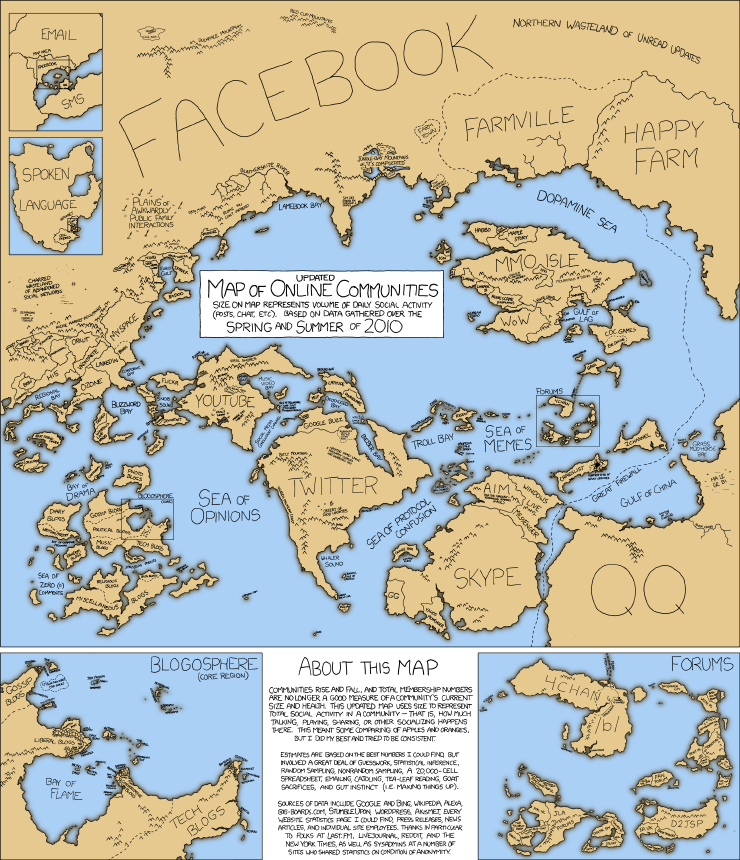
\includegraphics[height=\textheight]{../pics/online_communities_2}
\end{center}

\section{The Web as Corpus}


\myslide{The Web as Corpus}
\MyLogo{}
\begin{itemize}
\item the web is a collection of text, thus it is a corpus
\item the largest available corpus: more than $7.2 \times 10^{11}$ words 
\\ (10 times bigger than the English Gigaword Corpus) % [Liu and Curran 2006])
\item nearly all kinds of text and lots of languages present
\item not preprocessed, lots of ungrammatical (and linguistically useless) text
\item how to access it?
\end{itemize}

\myslide{Direct Query or Sample?}
\begin{itemize}
\item \blu{Direct Query}: Search Engine as Query tool and WWW as corpus
\\  (Objection: Results are not reliable)
\begin{itemize}
\item Population and exact hit counts are unknown $\Rightarrow$ no statistics
possible.
\item Indexing does not allow us to draw conclusions on the data.
\item[\Bad] Search engines miss functionalities that linguists /
lexicographers would like to have (POS, lemmatization, \ldots).
\end{itemize}
\item \blu{Web Sample}: Use search engine to download data from the
net and build a corpus from it.
\begin{itemize}
\item known size and exact hit counts $\Rightarrow$ statistics possible.
\item people can draw conclusions over the included text types.
\item (limited) control over the content.
\item[\Bad] sparser data
\end{itemize}
\end{itemize}

\myslide{Direct Query}
\begin{itemize}
\item Document counts are shown to correlate directly with ``real'' frequencies
(Keller and Lapata, 2003), so search engines can help - but...
\item lots of repetitions of the same text (not representative)
\item very limited query precision (no upper/lower case, no punctuation...)
\item only estimated counts, often hard to reproduce exactly
\item how to access (Google API, Yahoo API, Scripts)
\item Alexa: ``buy'' (parts of) web, and process it on their machines
\end{itemize}

\myslide{Direct Query Example}
\begin{itemize}
\item Directly using web counts (instead of corpus counts), 
 \\  VerbOcean  (Chklovski \& Pantel 2004)
  \begin{itemize}
  \item gather verb pairs which are semantically related but the relation is unknown
    (DIRT: Lin and Pantel 2001)
    \\ example pair: \textit{love -- marry}
  \item pick a semantic relation (e.g. \iz{happens-before}) and design typical patterns
    for this relation (e.g. \textit{to X and then Y})
  \item instantiate the patterns (\textit{to love and then marry}) and count Google hits
    (here: 6)
  \item estimate whether or not the number of hits indicates a significant
    correlation, then assign the relation (or not)
  \end{itemize}
\end{itemize}

\myslide{VerbOcean}
\MyLogo{\url{http://demo.patrickpantel.com/demos/verbocean/}}

\begin{center}
  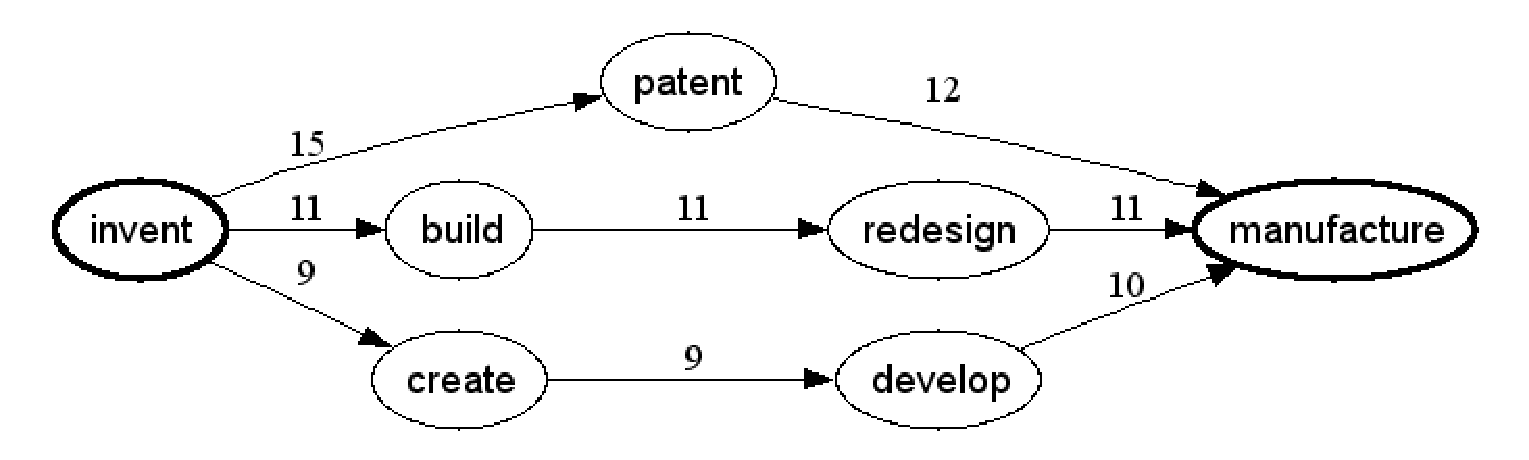
\includegraphics[width=\textwidth]{../pics/invent-manufacture-hb3}
\end{center}

% Mirella Lapata Web vs BNC
%\url{http://homepages.inf.ed.ac.uk/mlap/Papers/naacl04a.pdf}

%%%
%%% 

\myslide{Limitations of web search interfaces}

\begin{itemize}
\item Search engines only provide limited context
\item Search engines do not allow for linguistically complex
queries 
\item Results are organized according to relevance to the
topic, not to left/right context
\item Search engine counts cannot generally be trusted
\item Access may be limited to $n$ hits/second$\|$day
\end{itemize}



\myslide{Some Issues with Google Web Counts}
\MyLogo{\url{http://languagelog.ldc.upenn.edu/nll/?p=1943}}

Search for:
\begin{itemize}\addtolength{\itemsep}{-1ex}
\item machine \hfill ``machine''
\item machine machine
\item the machine
\item machine translation
\item ``machine translation''
\end{itemize}

\begin{quote}
  The bottom line, said Mr. Norvig, is that getting an accurate
  estimate isn't that important for most of Google's users, so the
  company hasn't invested much time and computing power. "\textit{It's only
  reporters and computational linguists who care if it's really
  precise}," he said.
\end{quote}

\myslide{Web Count Units}
\MyLogo{http://itre.cis.upenn.edu/~myl/languagelog/archives/000953.html}

\begin{itemize}\addtolength{\itemsep}{-1ex}
\item \blu{ghit} or ``google hit'' is the most common unit used to
  count web snippets (in the early 2000s)
  \begin{itemize}
  \item it is document frequency not term frequency
  \end{itemize}
\item \blu{whit} or ``web hit'' is the more general term
\item Normally you compare two phenomena to get a unitless ratio
  \\(e.g. \eng{different from} vs \eng{different than})
  \\ 251,000,000 ghits vs 71,500,000 or \emp{3.5:1} (accessed 2012-04-04)
%(/ 251 71.5) 3.5104895104895104
\item \blu{GPB}, for ``Ghits per billion documents'' is good if want a
  more stable number (suggested by Mark Liberman)
\\ but Google no longer releases the index size 
\item So always say when you counted, and try to use ratios
\end{itemize}

\myslide{Google Books Ngram Viewer}
\MyLogo{\url{http://www.gogeometry.com/software/google_ngram_mathematics_topology.html}}

\begin{center}
  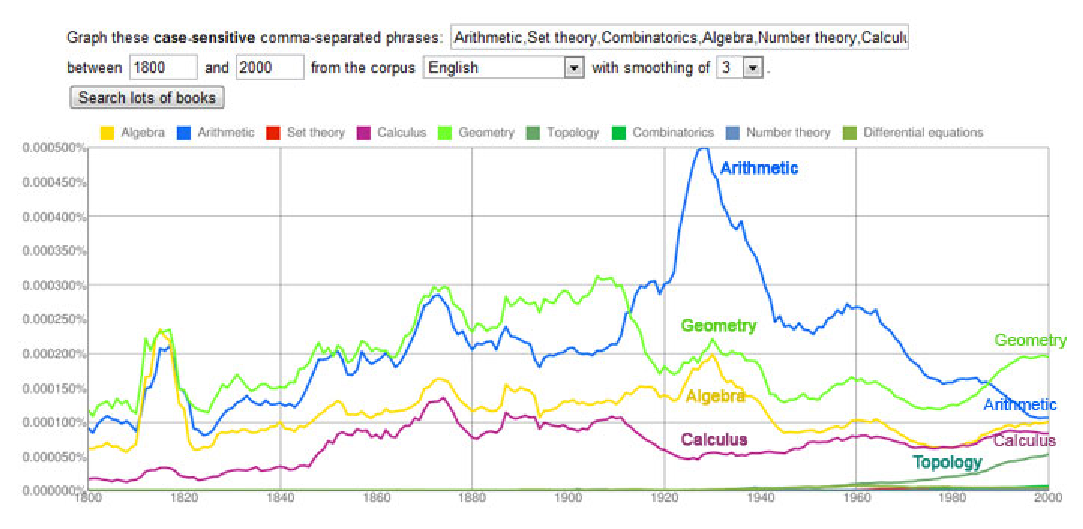
\includegraphics[width=\textwidth]{../pics/google_ngram_math_7}
\end{center}



\section{Google Books Ngram Viewer}
\MyLogo{\url{https://books.google.com/ngrams}}

\begin{itemize}
\item Display a graph showing how phrases have occurred in a corpus of books 
  \begin{itemize}
  \item A variety of corpora (different languages, different genres, different times)
  \end{itemize}
\item Can do various searches
  \begin{itemize}
  \item Wildcards: \eng{I like to *}
  \item Inflection: \eng{book\_INF a hotel}
  \item Simple POS
  \item You can do combinations: \eng{*\_NOUN rocks}; \eng{green\_*}
  \item Dependencies: \eng{has=$>$*\_NOUN}
  \end{itemize}
\end{itemize}

\myslide{Let's try it}

\begin{itemize}
\item Compare similar words (e.g. \eng{Miss} vs \eng{Mrs} vs \eng{Mdm} vs \eng{Ms})
\\ try some synonyms (\eng{poop, shit, \ldots})
\item Find common objects
\item Compare translation equivalents (\eng{eat} vs 吃 \eng{chi})
\end{itemize}



\section{Web Sample}
\myslide{Sample the Web}
\MyLogo{}
\begin{itemize}
\item Extracting and filtering web documents to create linguistically
  annotated corpora (Kilgarriff and Dhonnchadha, 2006)
  \begin{itemize}
  \item gather documents for different topics (balance!)
  \item exclude documents which cannot be preprocessed with available
    tools (here taggers and lemmatizers)
  \item exclude documents which seem irrelevant for a corpus (too short or
    too long, word lists,...)
  \item do this for several languages and make the corpora available
  \end{itemize}
\end{itemize}


\myslide{Internet Corpora: Outline}
\MyLogo{\url{http://corpus.leeds.ac.uk/internet.html}}

\begin{enumerate}
\item Select Seed Words (500)
\item Combine to form multiple queries (6,000)
\item Query a search engine and retrieve the URLs (50,000)
\item Download the files from the URLS (100,000,000 words)
\item Postprocess the data (encoding; cleanup; tagging and parsing)
\end{enumerate}

Sharoff, S (2006) Creating general-purpose corpora using automated search engine queries. In M. Baroni, S. Bernardini (eds.) \textit{WaCky! Working papers on the Web as Corpus}, Bologna, 2006.

\myslide{Internet Corpora}
\MyLogo{\url{http://corpus.leeds.ac.uk/internet.html}}
 
 \begin{description}
 \item [Select about 500 words] from a list of the most frequent word
   forms in your language. It is important that selected words are
   sufficiently general, i.e. they do not belong to a specific domain,
   but they are not function words. For instance, \textit{picture,
     extent, raised, events} are good query words for English.
 \item [Produce a list of 5000-6000 queries] each of which consists of
   4 words (you may need more to get more links). If the language for
   which you want to collect a corpus is not listed by Google yet, add
   a couple of very frequent function words that are not used in
   cognate languages. If you collect a corpus for a language with
   relatively few Internet pages, you may decrease the number of words
   in a query (however, this will also decrease the amount of
   connected text in the pages returned, so you'll get more price
   lists, forms, catalogues, etc). Collect the top 10 URLs produced by
   Google for each query.

 \item [Download URLs]. The list of successfully
   downloaded URLs constitutes an open-source corpus.  

 \item [Postprocess] the set of downloaded files --- correction of
   encodings, conversion of all texts to Unicode, filtering out
   duplicate pages, removing navigation frames, etc, followed by
   lemmatisation and part-of-speech tagging.
 \item [Composition assessment]: take a sample of about 200 texts from
   the corpus and describe them according to a text typology:
\blu{Authorship; Mode; Audience; Domain; Aim}.
 \item [Compare]: If you have another corpus for the same
   language, you can compare their frequency lists using the
   log-likelihood score (see Paul Rayson's Log-likelihood calculator)
 \end{description}


\myslide{Domain Specific Corpora}

\begin{itemize}
\item You can tune a web corpus in various ways
  \begin{itemize}
  \item adjusting the seed query terms (different content)
  \item restricting the URLs (e.g. only \url{.edu} or \url{.sg})
  \item restricting the page type (only blogs, \ldots)
  \item restricting the license of the web page \\ The English CC
    corpus has been compiled from webpages with the Creative Commons
    permissive licences. The corpus is less balanced than the main
    Internet-English (less professional news, more blogs and
    fanzines), but it can be redistributed without limitations.

  \end{itemize}
\end{itemize}



\myslide{Disposable Corpora}

 \begin{itemize}
  \item The web provides unprecedented opportunities for gathering data
  \item Viable source of ''disposable corpora”, built ad hoc for specific purposes
  \item Essential for working with specialized languages
  \item Need to automatically extract web corpus 
    \\ extraction is time-consuming
\end{itemize}

%\myslide{Internet Corpora: Demo}

\myslide{Post-processing}
\begin{itemize}
\item Filter documents by size
  \begin{itemize}
  \item Small documents ($<5KB$) contain very little real text
  \item Large documents ($>200KB$) tend to be indices, catalogues, lists, etc.
  \end{itemize}
\item Remove perfect duplicates
  \begin{itemize}
  \item Actually, removed both the original \& the duplicate:
  \item[\ldots] tend to be warning messages 
  \end{itemize}
\end{itemize}

\myslide{Boilerplate stripping}
\begin{itemize}
\item \blu{Boilerplate}: HTML markup, javascript, other non-linguistic
  material
\item Removing boilerplate information is crucial to obtaining
  linguistic data only
  \begin{itemize}
  \item Content-rich sections of a document will have a low 
    html tag density
  \item Boilerplate sections have a wealth of html
  \item This heuristic is ``relatively independent of language and
    crawling strategy''
  \end{itemize}
\item If a text does not have enough function words, it is likely
non-linguistic material (e.g., a list)
\begin{itemize}
\item Require at least 10 function word types and 30 tokens on a page
\item[\ldots]  which must make up at least 25\% of the total
words
\end{itemize}
\end{itemize}

\myslide{Near-duplicate detection}
\begin{itemize}
\item Take \blu{fingerprints} of a fixed number of randomly-selected $n$-grams (ignoring function words)
  \begin{itemize}
  \item e.g., extract 25 5-grams from each document
  \end{itemize}
\item Near-duplicates have a high overlap
 \begin{itemize}
 \item e.g., at least 2 5-grams in common
 \end{itemize}
\end{itemize}

%%% FIXME define ngrams

\myslide{Linguistic Post-processing}


\begin{itemize}
\item Prepare the  data  for searching:
  \begin{itemize}
  \item Run a POS tagger over it
  \item Clean the documents further, using POS tags
    \begin{itemize}
    \item Where the POS tag distribution is unusual,
    \item[\ldots] perform another round of anomalous document
finding
\item Look for problematic (erroneous) POS tags and
remove those documents
\item Use cues such as number of unrecognized words,
proporition of words with upper-case initial letters, \ldots
\end{itemize}
\end{itemize}
\item Index the document by word, POS and lemma
\end{itemize}

\myslide{Benefits of Web Corpora}

\begin{itemize}
\item Help address data sparseness issues
\item Provide more interpersonal material
\item Check the claims made with other corpora
\item Expensive to build corpora otherwise, yet they are
needed for under-resourced languages
\item Current corpora are often restricted in size and/or
variety
\item News corpora do not represent general language
\item Need a variety of text types
\end{itemize}

\myslide{Web Corpus Statistics}

\begin{tabular}{lrrrrr}
Corpus & tokens &  words &  lemmas &  URLs & words/doc \\
\hline
I-EN & 126,643,151 & 2,003,056 & 1,608,425 & 42,133 & 3,006 \\
I-DE & 126,117,984 & 3,384,491 & 3,081,197 & 31,195 & 4,043 \\
I-RU & 156,534,391 & 2,036,503 & 791,311 & 33,811 & 4,630
\end{tabular}

\myslide{British National Corpus (BNC)}

\begin{itemize}
\item 100-million-word text corpus
  \begin{itemize}
  \item 90\% written
  \item 10\% speech (transcribed)
  \end{itemize}
\item balanced across a wide variety of genres
\item  a representative sample of  British English of the late 20th century
\item POS tagging and domain/genre tagging
\end{itemize}

\begin{center}
  The corpus gold standard!
\end{center}

\myslide{Text assessment}
To determine whether the corpora is balanced like the BNC,
Sharoff assesses a variety of factors
\begin{itemize}
\item Authorship:
  \begin{itemize}
  \item Single
  \item Multiple
  \item Corporate: 44\% for I-EN, 18\% for BNC
  \item Unknown
  \end{itemize}
\item Gender: Female writers are underrepresented: 23\%/3\%
  male/female split in I-EN vs. 28\%/13\% for BNC
\newpage
\item Mode
  \begin{itemize}
  \item Written
  \item Spoken: 0-1\% for web corpora, 10\% for BNC
  \item Electronic: 16\% for Russian, 13\% for English, 9\% for
German; 0\% for BNC
\item Important type of data, as is similar to speech in some
ways, similar to writing in some
\end{itemize}
\item Audience
  \begin{itemize}
  \item General: 33\% in I-EN
  \item Informed: 45\% in I-EN
  \item Professional: 22\% in I-EN
  \end{itemize}
  Overall, I-EN seems somewhat balanced w.r.t. this
  classification (similar to BNC)
\item Aims of text production
  \begin{itemize}
  \item Discussion: 45\% in I-EN
  \item Recommendation (Hard to tell apart from discussion)
  \item Recreation: fiction=17\% in BNC vs. recreation=4\% in I-EN
  \item Instruction
  \item Information
  \end{itemize}
\item Domain
  \begin{itemize}
  \item natsci (natural sciences)
  \item appsci (applied sciences): 7\% in BNC vs. 29\% in I-EN
  \item socsci (social sciences): 16\% in RRC vs. 5\% in I-RU
  \item politics
  \item business
  \item life;  arts;  leisure
  \end{itemize}
\end{itemize}


\myslide{Corpus of web URLs}

\begin{itemize}
\item One strategy for releasing a corpus is to organize a list of
appropriate URLs
\item If a corpus consists of a list of URLs and associated
software for extracting them, how stable is such a corpus?
\item 
We can measure a corpus's half-life by seeing how
many pages are left after a certain amount of time
\item Initial experiments show that some links are gone after
a few months
\begin{itemize}
\item Feb 2005 → Aug 2005: 934/1000 remaining
\item Jun 2005 → Aug 2005: 982/1000 remaining
\end{itemize}
\item Need longer term studies and studies testing different
parameters
\end{itemize}

%%%
%%% Fixme add Lapata Stuff
%%%


\myslide{Some other corpora}

\begin{itemize}
\item \url{http://corpus.byu.edu/glowbe/}
\item \url{http://commoncrawl.org/}
\end{itemize}


\myslide{Summary}

\begin{itemize}
\item The web can be used as a corpus
  \begin{itemize}
  \item Direct access
    \begin{itemize}
    \item Fast and convenient
    \item Huge amounts of data
    \item[\Bad] unreliable counts 
    \end{itemize}
  \item Web sample
    \begin{itemize}
    \item Control over the sample
    \item Some setup costs (semi-automated)
    \item[\Bad] Less data 
    \end{itemize}
  \end{itemize}
\item Richer data than a compiled corpus
\item[\Bad] Less balanced
\end{itemize}

\myslide{References}

\begin{itemize}
\item Keller, Frank and Mirella Lapata. 2003. Using the Web to Obtain
  Frequencies for Unseen Bigrams. \textit{Computational Linguistics}
  29:3, 459-484.
\item Timothy Chklovski and Patrick Pantel. 2004. VERBOCEAN: Mining
  the Web for Fine-Grained Semantic Verb Relations. In
  \textit{Proceedings of Conference on Empirical Methods in Natural
    Language Processing (EMNLP-04)}. pp. 33-40. Barcelona, Spain.
\item Kilgarriff, Michael Rundell and Elaine Uí
  Dhonnchadha. 2006. Efficient corpus development for lexicography:
  building the New Corpus for Ireland. \textit{Language Resources and
    Evaluation Journal} 40 (2): 127-152.
\newpage
\item Lin, Dekang and Patrick Pantel. 2001. DIRT - Discovery of
  Inference Rules from Text. In \textit{Proceedings of ACM Conference on
  Knowledge Discovery and Data Mining (KDD-01)}. pp. 323-328. San
  Francisco, CA.
\item Sharoff, S (2006) Creating general-purpose corpora using automated search engine queries. In M. Baroni, S. Bernardini (eds.) \textit{WaCky! Working papers on the Web as Corpus}, Bologna, 2006.

\end{itemize}

%% 
%% Future
%%

\end{document}


%%% Local Variables: 
%%% coding: utf-8
%%% mode: latex
%%% TeX-PDF-mode: t
%%% TeX-engine: xetex
%%% End: 
